


\documentclass[conference]{IEEEtran}

\usepackage{acronym}

\usepackage{array}
\usepackage{multirow}
\usepackage{xspace}
\usepackage{url}
%\usepackage[dvips]{color}
\usepackage{subfigure}
\usepackage{pgf}
\usepackage{pgfplots,pgfplotstable} %for plotting results
\usepgfplotslibrary{units}
\usepackage{amsmath}
\usepackage{amsfonts,amssymb}
\usepackage{mathrsfs}
\usepackage{filecontents}
\usepackage{tikz} % for drawing
\usetikzlibrary{arrows,shapes,fit,automata,positioning,decorations,calc} % for drawing
\usetikzlibrary{spy,backgrounds}
\usepackage{algorithmic, algorithm}
\newcounter{lemmas}
\newtheorem{lemma}{Lemma}
%\newcounter{proofs}
%\newtheorem{proof}{Proof}
\newcounter{theorems}
\newtheorem{theorem}{Theorem}


%\newtheorem*{proof*}{Theorem}
%\newtheorem*{proof}{Proof}



\newcounter{definitions}
\newtheorem{definition}{Definition}


\newcommand{\ignore}[1]{{}}
\newcommand{\ourTool}{Piha\xspace}
\newcommand{\simulink}{Simulink\textsuperscript{\textregistered}\xspace}
\newcommand{\compiler}{Microsoft Visual C++\xspace}
\newcommand{\iSignal}{\tau} %internal signal for HA
\newcommand{\inSignal}[1]{#1~} %input signal for HA
\newcommand{\outSignal}[1]{#1~} %output signal from HA

\newcolumntype{L}[1]{>{\raggedright\let\newline\\\arraybackslash\hspace{0pt}}m{#1}}
\newcolumntype{C}[1]{>{\centering\let\newline\\\arraybackslash\hspace{0pt}}m{#1}}
\newcolumntype{R}[1]{>{\raggedleft\let\newline\\\arraybackslash\hspace{0pt}}m{#1}}
  %Macros/#defs for the paper

\begin{document}
	
		\renewcommand\floatpagefraction{.9}
		\renewcommand\dblfloatpagefraction{.95} % for two column documents
		\renewcommand\topfraction{.95}
		\renewcommand\dbltopfraction{.95} % for two column documents
		\renewcommand\bottomfraction{.95}
		\renewcommand\textfraction{.1}   
		\setcounter{totalnumber}{50}
		\setcounter{topnumber}{50}
		\setcounter{bottomnumber}{50}
		
		\setlength{\abovecaptionskip}{0pt}
		
		
\acrodef{CPS}{Cyber-Physical System}
\acrodef{DSP}{Digital Signal Processor}
\acrodef{DTTS}{Discrete Time Transition System}
\acrodef{DHA}{Deterministic Hybrid Automata}
\acrodef{EA}{Evolutionary Algorithm}
\acrodef{HIOA}{Hybrid Input Output Automata}
\acrodef{ILP}{Integer Linear Programming}
\acrodef{MCU}{Microcontroller Unit}
\acrodef{ODE}{Ordinary Differential Equation}
\acrodef{PoC}{Plant-on-a-Chip}
\acrodef{SHIOA}{Synchronous Hybrid Input Output Automata}
\acrodef{SWA}{Synchronous Witness Automata}
\acrodef{WHA}{Well-formed Hybrid Automata}
\acrodef{WCET}{Worst-Case Execution Time}
\acrodef{FSM}{Finite State Machine}

\acrodef{ST}{Stimulated}
\acrodef{UP}{Upstroke}
\acrodef{ERP}{Effective Refractory Period}
\acrodef{RRP}{Relative Refractory Period}
\acrodef{RP}{Resting Period}
\acrodef{AP}{Action Potential}

\acrodef{SA}{Sinoatrial}
\acrodef{AV}{Atrioventicular}
\acrodef{RVA}{Right Ventricular Apex}


\acrodef{NHN}{Network of Heart Nodes}
\acrodef{WH}{Water Heating System}
\acrodef{MTG}{Multiple Train Gate}
\acrodef{TSN}{Thermostat Network}
\acrodef{NP}{Nuclear Plant control}
 		%acronyms
	
\title{Hybrid automata models of the heart for formal verification of cardiac pacemakers \vspace{-0.5cm} }

\author{

	\vspace{-1cm}
}





\maketitle





\begin{abstract}

\end{abstract}


%%% Local Variables:
%%% mode: latex
%%% TeX-master: "../DATE2016_codegen"
%%% End:


\section{Introduction}

Artificial cardiac pacemakers are embedded devices that 
stimulate the heart with electrical impulses to 
maintain or restore a normal rhythm in people with slow heart rhythms.
These devices continuously monitor a human heart and must operate in a 
fail-safe manner all the time. 
However, in 1990-2000, close to 200,000 pacemakers were 
recalled due to software related failures~\cite{alemzadeh13}.
As the complexity of the pacemakers increase, there is a need for the
development of better processes for validation of such
medical devices.




\begin{figure}[bthp]
  \centering \scalebox{0.7}{ % Define block styles
\tikzstyle{process} = [rectangle, draw, fill=blue!15, 
text width=9em, text centered, rounded corners, minimum height=6em, text width=4.6em]
\tikzstyle{line} = [draw, -latex', ultra thick]


\begin{tikzpicture}
% Place nodes

%-----------------------------------------------------------------------
\node [process, fill=red!10] (HM) {Heart Model};
\node [process, right of = HM, fill=red!20,  node distance = 4.3cm] (Int) {Interface};
\node [process, right of = Int, fill=red!30, node distance = 4.3cm] (PM) {Pacemaker};

%-----------------------------------------------------------------------




%\node[draw, dashed, inner sep=0.2cm,
%	label={[label distance=0cm]60:Section~\ref{sec:SHA}}, 
%	fit= (GFSM)(CC)] (S3) {};

%--------------------------------------------------------------------------------
%edges
\draw [line] (HM.40) -- (Int.140) node[midway, above,text width=2cm]
{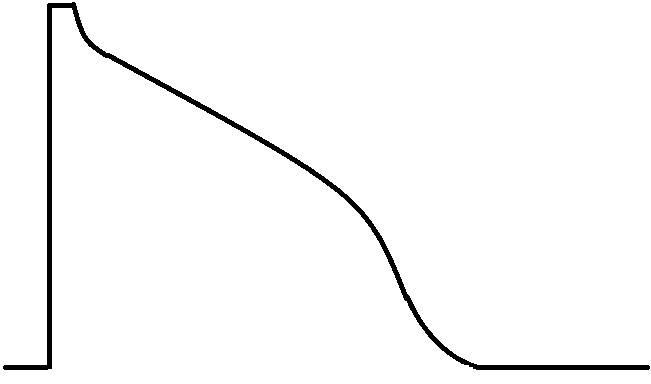
\includegraphics[scale=0.1]{figures/APicon}  Action Potentials };
\draw [line] (Int.40) -- (PM.140) node[midway, above,text width=2cm]
{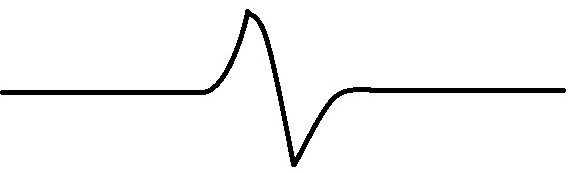
\includegraphics[scale=0.1]{figures/EGMicon} \acf{EGM}};
\draw [line] (PM.220) -- (Int.-40) node[midway, below,text width=2cm]
{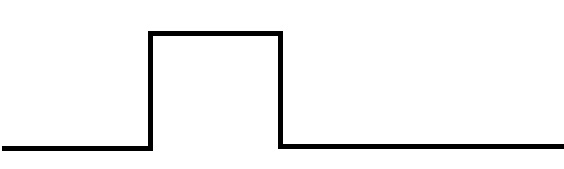
\includegraphics[scale=0.1]{figures/SQRicon} {Pacing}};
\draw [line] (Int.220) -- (HM.-40) node[midway, below,text width=2cm]
{Pacing};



\end{tikzpicture}     }
  \caption{Overview of the proposed modular code generation
    approach \label{fig:overview}}
\end{figure}

\begin{figure*}[hbpt]
  \centering {
	\centering
	\subfigure[\label{fig:heart} Diagram of the heart. Reproduced 
	from~\cite{zhihao12}]{
       \framebox[0.31\textwidth]{
				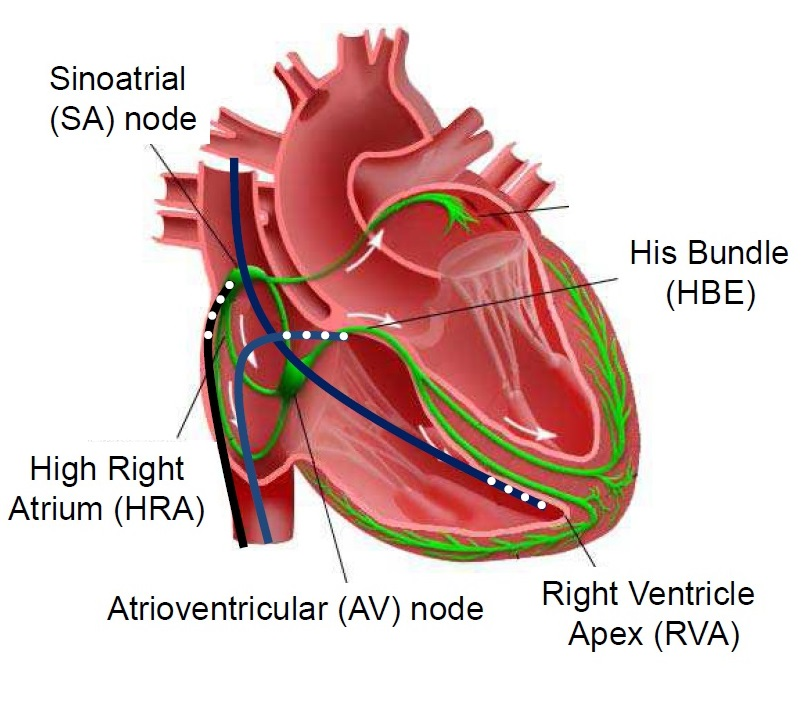
\includegraphics[width=0.262\linewidth]{figures/heart}
		} %framebox
	}
	\subfigure[The four stages of an \acf{AP}]{
		\framebox[0.31\textwidth]{
			\begin{tikzpicture}[transform shape, xscale=0.6, yscale=0.6]
\begin{axis}
[ xlabel={Time (ms)},
ylabel={Potential ({mV})},
axis y line = left,
axis x line = bottom,
xmin=0,   xmax=300,
ymin=0,   ymax=150,
ytick={0, 30, 44.5, 50, 100, 131.1, 150},
yticklabels={0, $v_R$, $v_T$, 50, 100, $v_O$, 150},
extra tick style={grid=major},
width=8.5cm,
height=6.5cm,
]
\addplot[color=blue!90,
mark=.,
mark size=2,
smooth,
const plot
]
table [x=t, y=v, col sep=comma] {./figures/actionPotentialData.csv};

\addplot[color=black!90,
dashed,
mark=.,
mark size=2
] coordinates {
	(0,30)
	(240,30)
};

\addplot[color=black!90,
dashed,
mark=.,
mark size=2
] coordinates {
	(0,44.5)
	(50,44.5)
};

\addplot[color=black!90,
dashed,
mark=.,
mark size=2
] coordinates {
	(0,131.1)
	(50,131.1)
};

\end{axis}

\tikzstyle{every state}=[rectangle, text centered, draw=none,text=black, draw,line width=0.3mm]

\node[state, shift={(0.2, -1.5)}, fill=green!20, inner xsep=0.0cm, minimum width=0.6cm] {RP};
\node[state, shift={(0.85, -1.5)}, fill=yellow!20, minimum width=0.5cm] {ST};
\node[state, shift={(3.00, -1.5)}, fill=red!20, minimum width=2.8cm] {ERP};
\node[state, shift={(1.50, -1.5)}, fill=blue!20, minimum width=0.5cm] {UP};
\node[state, shift={(5.15, -1.5)}, fill=green!20, minimum width=1.5cm] {RRP};
\node[state, shift={(6.40, -1.5)}, fill=green!20, minimum width=1cm] {RP};

\end{tikzpicture}
			\label{fig:actionPotential}
		}
	}
	\subfigure[An abstracted model of the conduction system]{ 
          \framebox[0.31\textwidth]{
          	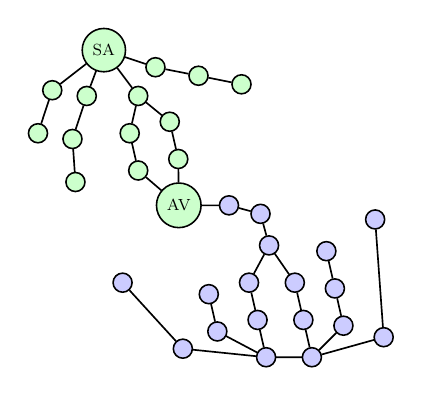
\begin{tikzpicture}[->,>=stealth',semithick,scale=0.73, transform shape]

\tikzstyle{every state}=[fill=blue!20,circle,minimum size=0.1cm]

\tikzset{
	atrialCell/.style={
		fill=green!20,
		circle,
		minimum size=0.1cm,
		draw,
		line width=0.2mm
	}
}

\tikzset{
	ventricularCell/.style={
		fill=blue!20,
		circle,
		minimum size=0.1cm,
		draw,
		line width=0.2mm
	}
}

\tikzset{
	autorhythmicCell/.style={
		fill=yellow!20,
		circle,
		minimum size=0.1cm,
		draw,
		line width=0.2mm
	}
}

\draw node[atrialCell](SA) {\footnotesize SA};

\node[atrialCell](CT) [below left=0.3cm and 0.5cm of SA] {};
\node[atrialCell](CT1) [below left=0.5cm and 0cm of CT] {};

\node[atrialCell](BB) [below right=-0.1cm and 0.5cm of SA] {};
\node[atrialCell](LA) [below right=-0.1cm and 0.5cm of BB] {};
\node[atrialCell](LA1) [below right=-0.1cm and 0.5cm of LA] {};

\node[atrialCell](RA) [below left=0.4cm and -0.1cm of SA] {};
\node[atrialCell](RA1) [below left=0.5cm and 0cm of RA] {};
\node[atrialCell](CS) [below left=0.5cm and -0.3cm of RA1] {};

\node[atrialCell](OS) [below right=0.4cm and 0.2cm of SA] {};
\node[atrialCell](Fast) [below left=0.4cm and -0.1cm of OS] {};
\node[atrialCell](Fast1) [below right=0.4cm and -0.1cm of Fast] {};
\node[atrialCell](Slow) [below right=0.2cm and 0.3cm of OS] {};
\node[atrialCell](Slow1) [below right=0.4cm and -0.1cm of Slow] {};
\node[atrialCell](AV) [below right=0.2cm and 0.3cm of Fast1] {\footnotesize AV};

\node[ventricularCell](His) [right=0.3cm of AV] {};
\node[ventricularCell](His1) [below right=-0.1cm and 0.3cm of His] {};
\node[ventricularCell](His2) [below right=0.3cm and -0.1cm of His1] {};

\node[ventricularCell](RBB) [below left=0.4cm and 0.1cm of His2] {};
\node[ventricularCell](RBB1) [below right=0.4cm and -0.1cm of RBB] {};
\node[ventricularCell](RVA) [below right=0.4cm and -0.1cm of RBB1] {};

\node[ventricularCell](LBB) [below right=0.4cm and 0.2cm of His2] {};
\node[ventricularCell](LBB1) [below right=0.4cm and -0.1cm of LBB] {};
\node[ventricularCell](LVA) [below right=0.4cm and -0.1cm of LBB1] {};

\node[ventricularCell](LVS) [above right=0.3cm and 0.3cm of LVA] {};
\node[ventricularCell](LVS1) [above left=0.4cm and -0.1cm of LVS] {};
\node[ventricularCell](CSLV) [above left=0.4cm and -0.1cm of LVS1] {};

\node[ventricularCell](LV) [above right=0.1cm and 1.0cm of LVA] {};
\node[ventricularCell](LV1) [above left=1.8cm and -0.1cm of LV] {};

\node[ventricularCell](RVS) [above left=0.2cm and 0.6cm of RVA] {};
\node[ventricularCell](RVS1) [above left=0.4cm and -0.1cm of RVS] {};

\node[ventricularCell](RV) [above left=-0.1cm and 1.2cm of RVA] {};
\node[ventricularCell](RV1) [above left=0.9cm and 0.8cm of RV] {};

\path[-] (SA) edge (BB);
\path[-] (BB) edge (LA);
\path[-] (LA) edge (LA1);

\path[-] (SA) edge (CT);
\path[-] (CT) edge (CT1);

\path[-] (SA) edge (RA);
\path[-] (RA) edge (RA1);
\path[-] (RA1) edge (CS);

\path[-] (SA) edge (OS);
\path[-] (OS) edge (Fast);
\path[-] (Fast) edge (Fast1);
\path[-] (OS) edge (Slow);
\path[-] (Slow) edge (Slow1);
\path[-] (Fast1) edge (AV);
\path[-] (Slow1) edge (AV);

\path[-] (AV) edge (His);
\path[-] (His) edge (His1);
\path[-] (His1) edge (His2);
\path[-] (His2) edge (RBB);
\path[-] (RBB) edge (RBB1);
\path[-] (RBB1) edge (RVA);
\path[-] (His2) edge (LBB);
\path[-] (LBB) edge (LBB1);
\path[-] (LBB1) edge (LVA);
\path[-] (RVA) edge (LVA);

\path[-] (RVA) edge (RVS);
\path[-] (RVS) edge (RVS1);

\path[-] (RVA) edge (RV);
\path[-] (RV) edge (RV1);

\path[-] (LVA) edge (LVS);
\path[-] (LVS) edge (LVS1);
\path[-] (LVS1) edge (CSLV);

\path[-] (LVA) edge (LV);
\path[-] (LV) edge (LV1);

\end{tikzpicture}
          	\label{fig:heartNetwork} 
	  } %framebox
	}

}
  \caption{Electrical conduction systems of the heart}
  \label{fig:heartOverview}
\end{figure*}

\textbf{Contributions} of the paper are:  



%%% Local Variables:
%%% mode: latex
%%% TeX-master: "../DATE2016_codegen"
%%% End:

\section{Background--the human heart }

Using Figure~\ref{fig:heartOverview}, we describe the
electrical conduction system of the heart.
% \noindent \textbf{Heart.}
The human heart (see Figure~\ref{fig:heart}) is a biological pump that
is essential for blood circulation using its rhythmic pumping activity.
It achieves this by regularly contracting and relaxing its muscles,
which is orchestrated through flow of electrical signals along a set of
cellular groups called nodes and associated paths called its
\emph{conduction system}. The source of the signal is a natural pacemaker in the left ventricle, called the \ac{SA} node, which triggers
automatically. First, this signal travels through the left and right
atria, contracting the muscles and pushing the blood into the
ventricles.

Second, to ensure both ventricles are filled, the \ac{AV} node
introduces critical delay in the conduction system. Finally, the
electrical signal propagates through both ventricles. This contracts the
muscles and pumps the blood out of the heart.

\noindent \textbf{\acf{AP}.} The propagation of electrical signals at
the cellular / nodal level is described as a change in voltage across
the cell membrane due to ionic flow. Over a period of time, this change
is depicted as the \acf{AP}~\cite{chen14} (see 
Figure~\ref{fig:actionPotential}). It can be described in four
stages.
\begin{enumerate}
\item \acf{RP}: This is the steady state, when the node is awaiting
  activation by an external stimulus.
\item \acf{ST}: When the external stimulus is above a threshold voltage ($V_T$).
\item \acf{UP}: After continuous stimulation, the cell's voltage 
	reaches the threshold voltage ($V_T$. This causes   the node to
  depolarises (inward flow of positive ions) and contracts the
  muscles. This depolarisation yields a stimulus that activates
  neighbouring nodes.
\item \acf{ERP}: Once activated, the node cannot be activated again due
  to the recovery process of the ionic channels. Any new stimulus will
  be blocked during this refractory period.
\end{enumerate}
Finally, the ionic channels will partially
recover (\acf{RRP}) and then fully recover (\ac{RP}). 
If activated again by
external stimulus during \ac{RRP}, the morphology
of the \ac{AP} will be shorter when compared to \ac{RP}.

\noindent \textbf{Abstract model.} The human heart has over two trillion
cells. For analytical purposes, a model consisting of a network of $33$~nodes 
is presented in literature and is used for testing off-the-shelf
pacemakers~\cite{zhihao12,chen14}. The abstracted electrical conduction
system consisting of nodes and paths is presented in
Figure~\ref{fig:heartNetwork}. The functionality of each node is
described using \acf{HIOA} in Section~\ref{sec:HA}.  During implementation, the 
connections between nodes are implemented as buffers where the length of the 
buffer depends on the conduction delay and step size.  Later in 
Section~\ref{sec:codeGen}, we use this network of nodes to illustrate our 
modular code generation.



%%% Local Variables:
%%% mode: latex
%%% TeX-master: "../DATE2016_codegen"
%%% End:

\section{Existing Heart models }
\label{sec:existingHeartModels}

\section{Proposed Heart models  }
\label{sec:proposedHeartModels}

\section{Verification of pacemakers }
\label{sec:verification}


\section{Benchmarking}
\label{sec:benchmarking}

We present a set of experiments to evaluate the efficacy 
\input{content/06_relatedWork}
\section{Conclusions}



\bibliographystyle{ieeetr}
\bibliography{references} 

\end{document}


